% Copyright 2016 - 2018 Bas van Meerten and Wouter Franssen
%
%This file is part of ssNake.
%
%ssNake is free software: you can redistribute it and/or modify
%it under the terms of the GNU General Public License as published by
%the Free Software Foundation, either version 3 of the License, or
%(at your option) any later version.
%
%ssNake is distributed in the hope that it will be useful,
%but WITHOUT ANY WARRANTY; without even the implied warranty of
%MERCHANTABILITY or FITNESS FOR A PARTICULAR PURPOSE.  See the
%GNU General Public License for more details.
%
%You should have received a copy of the GNU General Public License
%along with ssNake. If not, see <http://www.gnu.org/licenses/>.

\documentclass[11pt,a4paper]{article}
% Copyright 2016 - 2017 Bas van Meerten and Wouter Franssen
%
%This file is part of ssNake.
%
%ssNake is free software: you can redistribute it and/or modify
%it under the terms of the GNU General Public License as published by
%the Free Software Foundation, either version 3 of the License, or
%(at your option) any later version.
%
%ssNake is distributed in the hope that it will be useful,
%but WITHOUT ANY WARRANTY; without even the implied warranty of
%MERCHANTABILITY or FITNESS FOR A PARTICULAR PURPOSE.  See the
%GNU General Public License for more details.
%
%You should have received a copy of the GNU General Public License
%along with ssNake. If not, see <http://www.gnu.org/licenses/>.

\usepackage[british]{babel}
\usepackage{graphicx,booktabs,listings,amsmath,pgfplots,pgfplotstable}
\usepackage[small,bf,nooneline]{caption}
\usepackage{subcaption}
\usepackage[sort&compress,numbers]{natbib}
\usepackage{tikz}
\usepackage{mathtools}
\usepackage[nottoc]{tocbibind}%adds bibliography to table of contents.
\graphicspath{{./images/}}
%\setlength{\textwidth}{453pt} %597 pt is the a4 paperwidth. Minus 2 in margin. 72 pt = 1 in
%\setlength{\hoffset}{-\oddsidemargin}
%\setlength{\voffset}{-30pt} %
%\setlength{\textheight}{651 pt} %a4 height 845 pt minus 2* total headheight. In this case 2*88pt
%% examine margines via the layout package. Use command \layout{} in document to draw a picture.
%\setlength{\parindent}{0.5 cm}
%\setlength{\parskip}{0 cm}
\usepackage[left=82pt,right=82pt,top=95pt,bottom=95pt,footnotesep=0.5cm]{geometry}
%\setlength{\headheight}{14pt}

%define colours--------------------
%dark
\usepackage{xcolor}
\definecolor{MyGrayD}{RGB}{1,1,1}
\definecolor{MyRedD}{RGB}{237,45,46}
\definecolor{MyGreenD}{RGB}{0,140,71}
\definecolor{MyBlueD}{RGB}{24,89,169}
\definecolor{MyOrangeD}{RGB}{243,125,34}
\definecolor{MyPurpleD}{RGB}{102,44,145}
\definecolor{MyBrownD}{RGB}{161,29,32}
\definecolor{MyPinkD}{RGB}{179,56,147}
%normal
\definecolor{MyGray}{RGB}{114,114,114}
\definecolor{MyRed}{RGB}{241,89,95}
\definecolor{MyGreen}{RGB}{121,195,106}
\definecolor{MyBlue}{RGB}{89,154,211}
\definecolor{MyOrange}{RGB}{249,166,90}
\definecolor{MyPurple}{RGB}{158,102,171}
\definecolor{MyBrown}{RGB}{205,112,88}
\definecolor{MyPink}{RGB}{215,127,179}
%light
\definecolor{MyGrayL}{RGB}{204,204,204}
\definecolor{MyRedL}{RGB}{242,174,172}
\definecolor{MyGreenL}{RGB}{216,228,170}
\definecolor{MyBlueL}{RGB}{184,210,235}
\definecolor{MyOrangeL}{RGB}{242,209,176}
\definecolor{MyPurpleL}{RGB}{212,178,211}
\definecolor{MyBrownL}{RGB}{221,184,169}
\definecolor{MyPinkL}{RGB}{235,191,217}
%----------------------------------

%Figure ref with hyperref
\newcommand{\fref}[1]{\hyperref[#1]{Figure \ref*{#1}}}
\newcommand{\sref}[1]{\hyperref[#1]{Section \ref*{#1}}}
\newcommand{\tref}[1]{\hyperref[#1]{Table \ref*{#1}}}

%Makes a new command for figures with input values: filename, width(times linewidth),
% caption and label.
\newcommand{\onefigure}[4]{
\setlength{\captionwidth}{#2\linewidth}
\begin{figure}
\includegraphics[width=#2\linewidth]{#1}
\centering
\parbox{\linewidth}{\caption{#3}
\label{#4}}
\end{figure}
}

%Makes a new command for tikz figures with input values: tikz commands, 
% caption and label.
\newcommand{\onetikz}[3]{
\settowidth{\captionwidth}{#1}
\ifthenelse{\lengthtest{\captionwidth<0.7\linewidth}}{\setlength{\captionwidth}{0.7\linewidth}}{}

\begin{figure}
\centering
#1
\centering
\parbox{\linewidth}{\caption{#2}
\label{#3}}
\end{figure}
}

%Makes a new command for two figures next to each other with input values: filename1, caption1, label1,filename2, caption2 and label2. Figure width is set to 0.47\linewidth and the space between the figures is filled with \hfill so the sides of the figures align with to edge of the line.
\newcommand{\twofigure}[6]{
\setlength{\captionwidth}{\linewidth}
\begin{figure*}[ht!]
\begin{minipage}[t]{0.47\linewidth}
\includegraphics[width=\linewidth]{#1}
\centering
\caption{#2}
\label{#3}
\end{minipage}
\hfill
\begin{minipage}[t]{0.47\linewidth}
\centering
\includegraphics[width= \linewidth]{#4}
\centering
\caption{#5}
\label{#6}
\end{minipage}
\end{figure*}
}


%Makes a new command for a table with caption witdh equal to the total table width. Input: tabular, caption and label. Example:
%\onetable{
%\begin{tabular}{ccc}
%a&b&c\\
%\hline
%1&1&1\\
%1&1&1\\
%1&1&1\\
%\end{tabular}
%{The caption.}
%{tab:table1}
%}
\newcommand{\onetable}[3]{
\settowidth{\captionwidth}{#1}
\ifthenelse{\lengthtest{\captionwidth<0.7\linewidth}}{\setlength{\captionwidth}{0.7\linewidth}}{}
\begin{table}
\caption{#2}
\vspace{-0.24cm} %Puts caption close to toprule
\label{#3}
\centering
#1
\end{table}
}

%Makes a long table with captionwidth equal to tablewidth. It takes the following arguments:
%1: Column specifier (e.g. cccc)
%2: Caption
%3: Label
%4: First head (i.e. first row of regular table)
%5: Head of consecutive pages
%6: Foot of pagebreak
%7: Lastfoot (e.g. \midrule)
%8: Body of table
\newcommand{\onelongtable}[8]{
\begin{center}
\settowidth{\captionwidth}{
\begin{tabular}{#1}
#4
#8
\end{tabular}} % This ends the captionwidth part. Next comes the real table.

\begin{longtable}{#1}
\caption{#2}\\
\vspace{-0.74cm} %Puts caption close to toprule
\label{#3}\\

#4
\endfirsthead

#5
\endhead

#6
\endfoot

#7
\endlastfoot

#8
\end{longtable}
\end{center}}




%1:pgfplots code
%2:width
%3:caption
%4:label
\newcommand{\pgfplotsfigure}[4]{
\pgfplotsset{width=#2\linewidth}
\setlength{\captionwidth}{#2\linewidth}
\begin{figure}[t]
\centering
#1
\centering
\parbox{\linewidth}{\caption{#3}
\label{#4}}
\end{figure}
}


\usepackage[bitstream-charter]{mathdesign}
\usepackage[T1]{fontenc}
\usepackage[protrusion=true,expansion,tracking=true]{microtype}
\pgfplotsset{compat=1.7,/pgf/number format/1000 sep={}, axis lines*=left,axis line style={gray},every outer x axis line/.append style={-stealth'},every outer y axis line/.append style={-stealth'},tick label style={font=\small},label style={font=\small},legend style={font=\footnotesize}}
\usepackage{colortbl}
\usetikzlibrary{calc}

%Set section font
\usepackage{sectsty}
\allsectionsfont{\color{black!70}\fontfamily{SourceSansPro-LF}\selectfont}
%--------------------


%Set toc fonts
\usepackage{tocloft}
%\renewcommand\cftchapfont{\fontfamily{SourceSansPro-LF}\bfseries}
\renewcommand\cfttoctitlefont{\color{black!70}\Huge\fontfamily{SourceSansPro-LF}\bfseries}
\renewcommand\cftsecfont{\fontfamily{SourceSansPro-LF}\selectfont}
%\renewcommand\cftchappagefont{\fontfamily{SourceSansPro-LF}\bfseries}
\renewcommand\cftsecpagefont{\fontfamily{SourceSansPro-LF}\selectfont}
\renewcommand\cftsubsecfont{\fontfamily{SourceSansPro-LF}\selectfont}
\renewcommand\cftsubsecpagefont{\fontfamily{SourceSansPro-LF}\selectfont}
%--------------------

%Define header/foot
%\usepackage{fancyhdr}
%\pagestyle{fancy}
%\fancyhead[LE,RO]{\fontfamily{SourceSansPro-LF}\selectfont \thepage}
%\fancyhead[LO,RE]{\fontfamily{SourceSansPro-LF}\selectfont \leftmark}
%\fancyfoot[C]{}
%--------------------

%remove page number from first chapter page
%\makeatletter
%\let\ps@plain\ps@empty
%\makeatother
%----------------------

\usepackage[hidelinks,colorlinks,allcolors=black, pdftitle={MQMAS processing in ssNake},pdfauthor={Wouter M.J.\ Franssen}]{hyperref}

\interfootnotelinepenalty=10000 %prevents splitting of footnote over multiple pages
\linespread{1.2}

\title{\color{black}\fontfamily{SourceSansPro-LF}\bfseries MQMAS processing in ssNake}
\author{}
\date{\color{black}\fontfamily{SourceSansPro-LF}\bfseries \today}


\begin{document}
%\newgeometry{left=72pt,right=72pt,top=95pt,bottom=95pt,footnotesep=0.5cm}
\microtypesetup{protrusion=true} % enables protrusion

\maketitle

\section{Introduction}
The following will explain how Multiple Quantum Magic Angle spinning (MQMAS) NMR data can be processed in ssNake.
 The
tutorial delivered with the ssNake program is considered as prior knowledge. If you have not yet
studied this, please do so before continuing with this example.

MQMAS is a 2D experiment for half-integer quadrupolar nuclei which, after proper processing, leads to a spectrum with the regular
quadrupolar powder patterns along D2, and peaks at the `isotropic' value along D1. This allows the
separation of multiple overlapping quadrupolar sites on the basis of their `isotropic' value (which
is a combination of the isotropic chemical shift, and the isotropic quadrupolar shift, which is also called
the quadrupolar induced shift). 

The experiment is almost famously hard to process. Not because of
the complication of the steps involved, but due to the high number of different types of MQMAS experiments
and the different ways to process these. It is therefore impossible to give a full overview of all
the different approaches here, in this tutorial. However, an attempt is made to show a good way for
processing the data for both the regular type (shifting echo or $z$-filter) and the split t1 MQMAS
experiment.


\section{Data}
In this tutorial we will use two data sets, recorded for solid rubidium nitrate (RbNO$_3$). The
sets are for $^{87}$Rb $3Q$ MQMAS, with $z$-filter or and split t1. The
data was recorded on a 600 MHz Varian machine using 15 kHz MAS.


\section{\textit{z}-filter processing}
First, we will look into the processing of MQMAS data recorded using a $z$-filter experiment (also
called three pulse MQMAS). Note that data recorded with a regular two pulse MQMAS (the standard
MQMAS experiment) can be processed in an identical way.

Processing the data has the following steps:
\begin{itemize}
  \item Applying the hypercomplex operation (States)
  \item Processing of the direct dimensions D2 (zerofill, Fourier, apodize, phase)
  \item Processing of the indirect dimension D1 (zerofill, Fourier, apodize, phase)
  \item Shearing the spectrum
  \item Scaling the spectral width in the indirect dimension
  \item Referencing both dimensions
\end{itemize}

One of the tricky thing of MQMAS processing is that the different traces along D1, have signal
starting at different positions in the FID (along D2). When applying apodization, the centre of the
apodization widow must be shifted differently for each trace along D1.


\begin{itemize}
	\item Open the Varian file Rb87\_3Q\_Zf.fid using File $\longrightarrow$ Open
	\item Set the view to D1 (sideframe, radiobutton)
	\item Convert the hypercomplex data via Transforms  $\longrightarrow$ Hypercomplex  $\longrightarrow$
	  States
	\item Set the view to D2 (sideframe, radiobutton)
\end{itemize}
Now, we will apply some apodization. Note that in this case, the position of the echo maximum shift
as a function of the D1 time. This must be taken into account when applying the apodization, and is
often called `shifting echo' apodization.

\begin{itemize}
	\item Open the Apodization window via Tools $\longrightarrow$ Apodize
 \item Set Gaussian at 80
 \item Set Shifting to `Spin 3/2, -3Q'. This sets the shifting to 7/9 i.e. 0.7778
 \item Press Ok to apply.
\end{itemize}
This should show:
\begin{center}
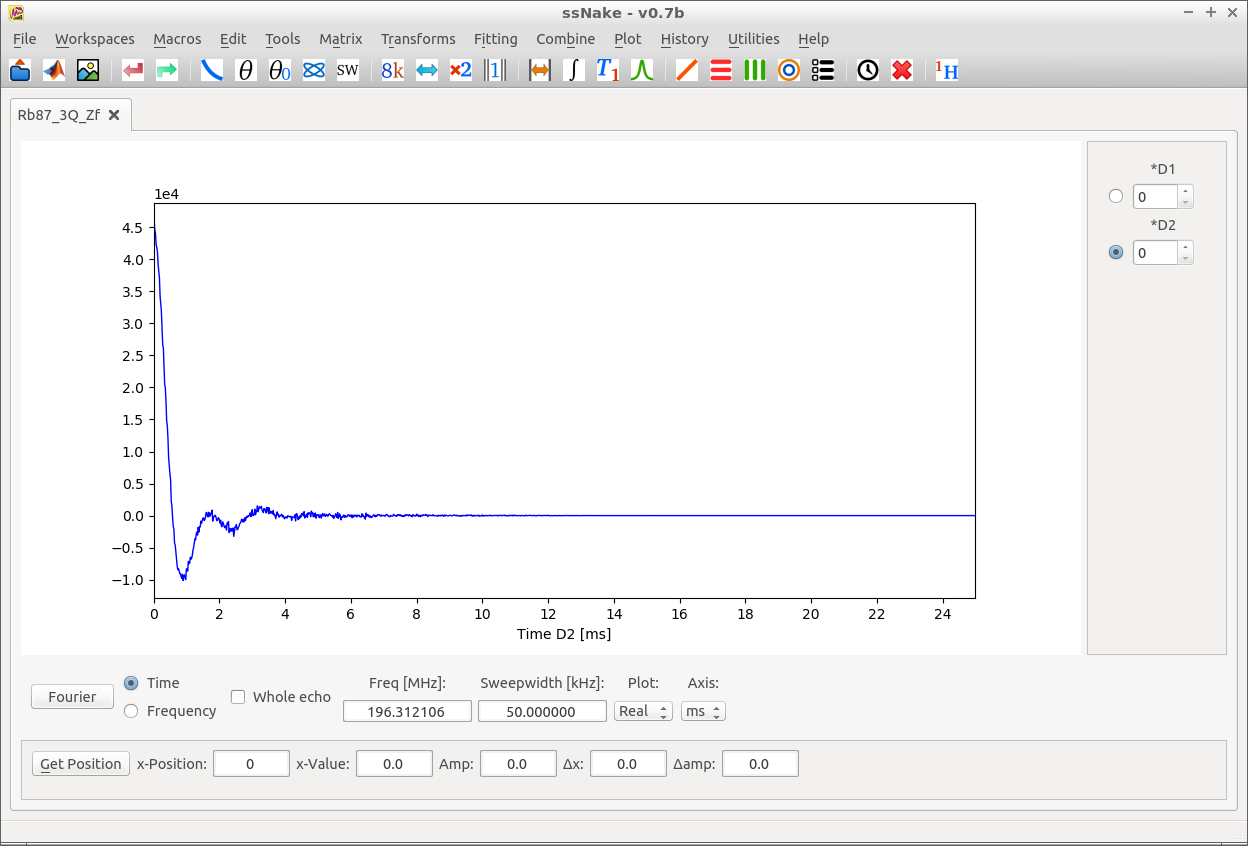
\includegraphics[width=0.8\linewidth]{Figs/Fig1.png}
\end{center}

\begin{itemize}
	\item Fourier Transform
	\item Phase with 2.5 degrees 0 order phasing (Tools  $\longrightarrow$ Phasing)
\end{itemize}

This should show:
\begin{center}
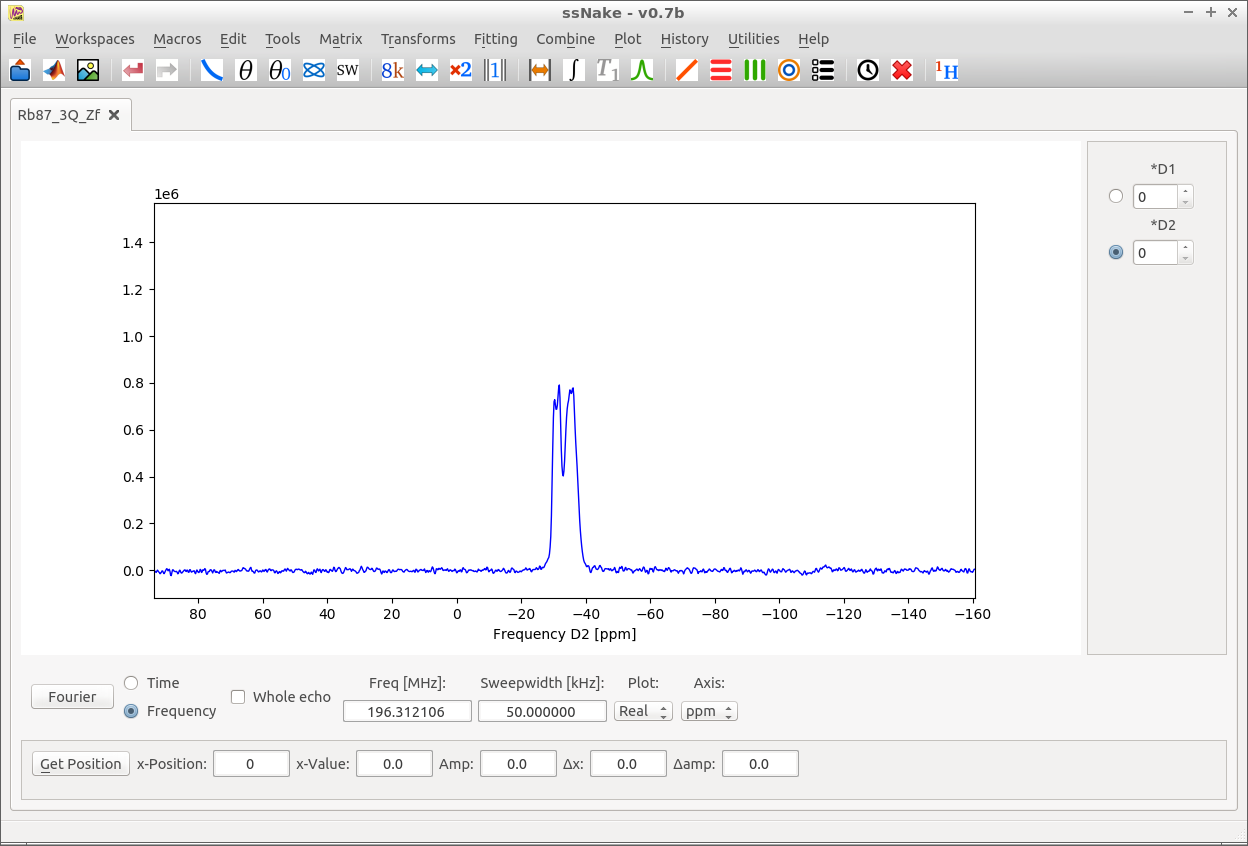
\includegraphics[width=0.8\linewidth]{Figs/Fig2.png}
\end{center}
A nice quadrupolar spectrum.

Now, we must process the indirect dimension (D1):
\begin{itemize}
	\item Switch to D1 (sideframe, radiobutton), and select data point 614 in D2.
	\item Do a complex conjugate (Tools $\longrightarrow$ Complex Conjugate)\footnote{The Varian data
	  we loaded has a different complex definition, so a conjugate in the indirect dimension is
	nearly always needed.}
\end{itemize}
This should show:
\begin{center}
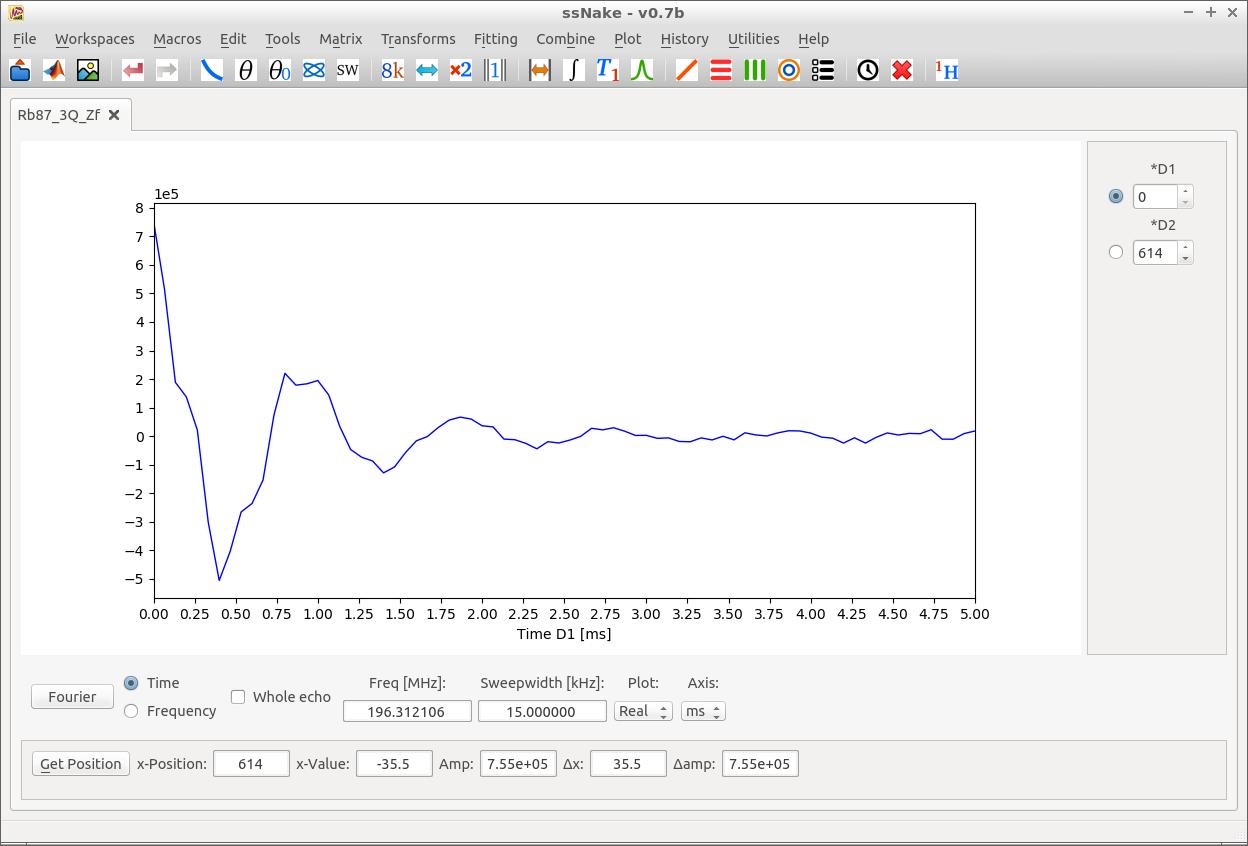
\includegraphics[width=0.8\linewidth]{Figs/Fig3.png}
\end{center}
Now we need some zerofilling etc.:
\begin{itemize}
	\item Set the size to 1024 points (Matrix $\longrightarrow$ Sizing)
	\item Fourier Transform
\end{itemize}
This gives the spectrum along D1 for this trace:
\begin{center}
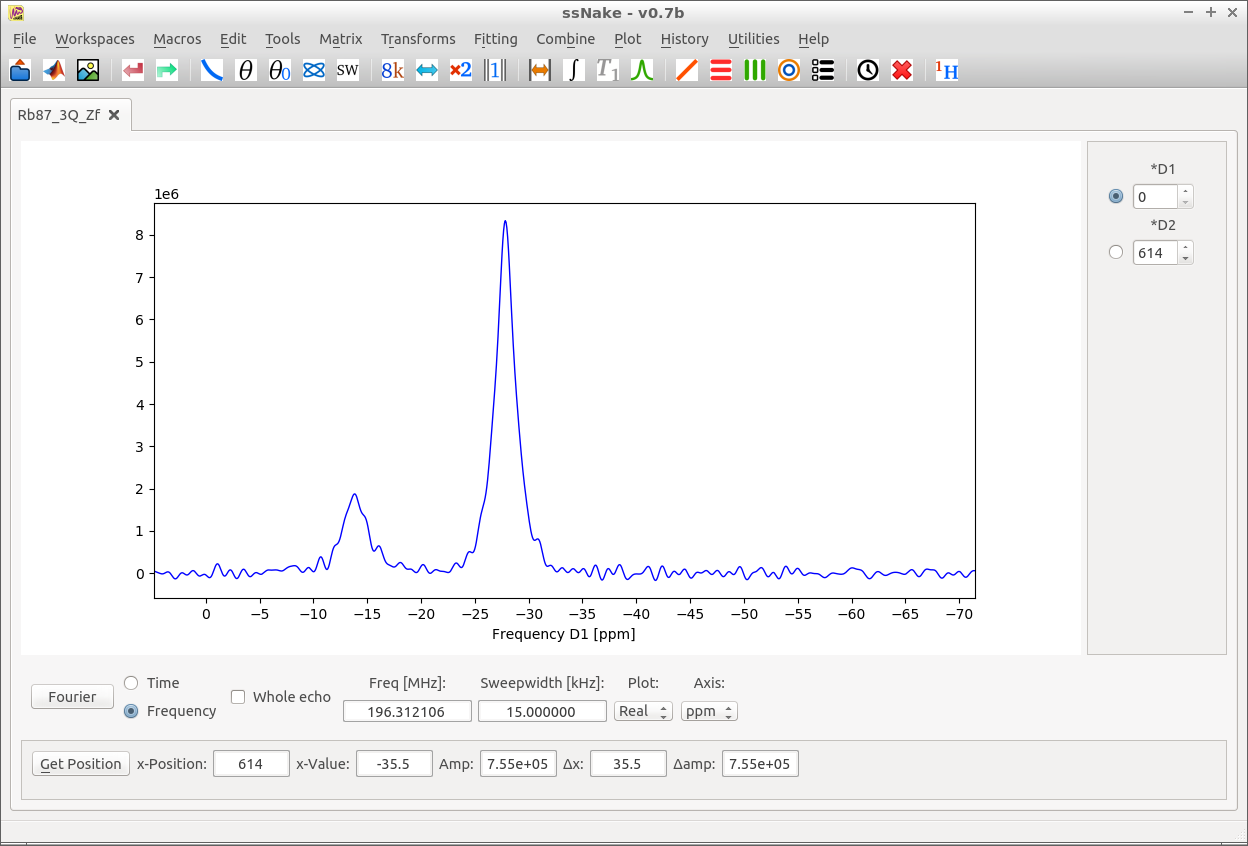
\includegraphics[width=0.8\linewidth]{Figs/Fig4.png}
\end{center}
The phasing looks good, so we do not need to do that.

We have now processed both dimensions, so we can view the data as a contour plot:
\begin{itemize}
	\item Switch to D2 (sideframe, radiobutton)
	\item Change the view to a contour plot: Plot  $\longrightarrow$ Contour
\end{itemize}
We now have:
\begin{center}
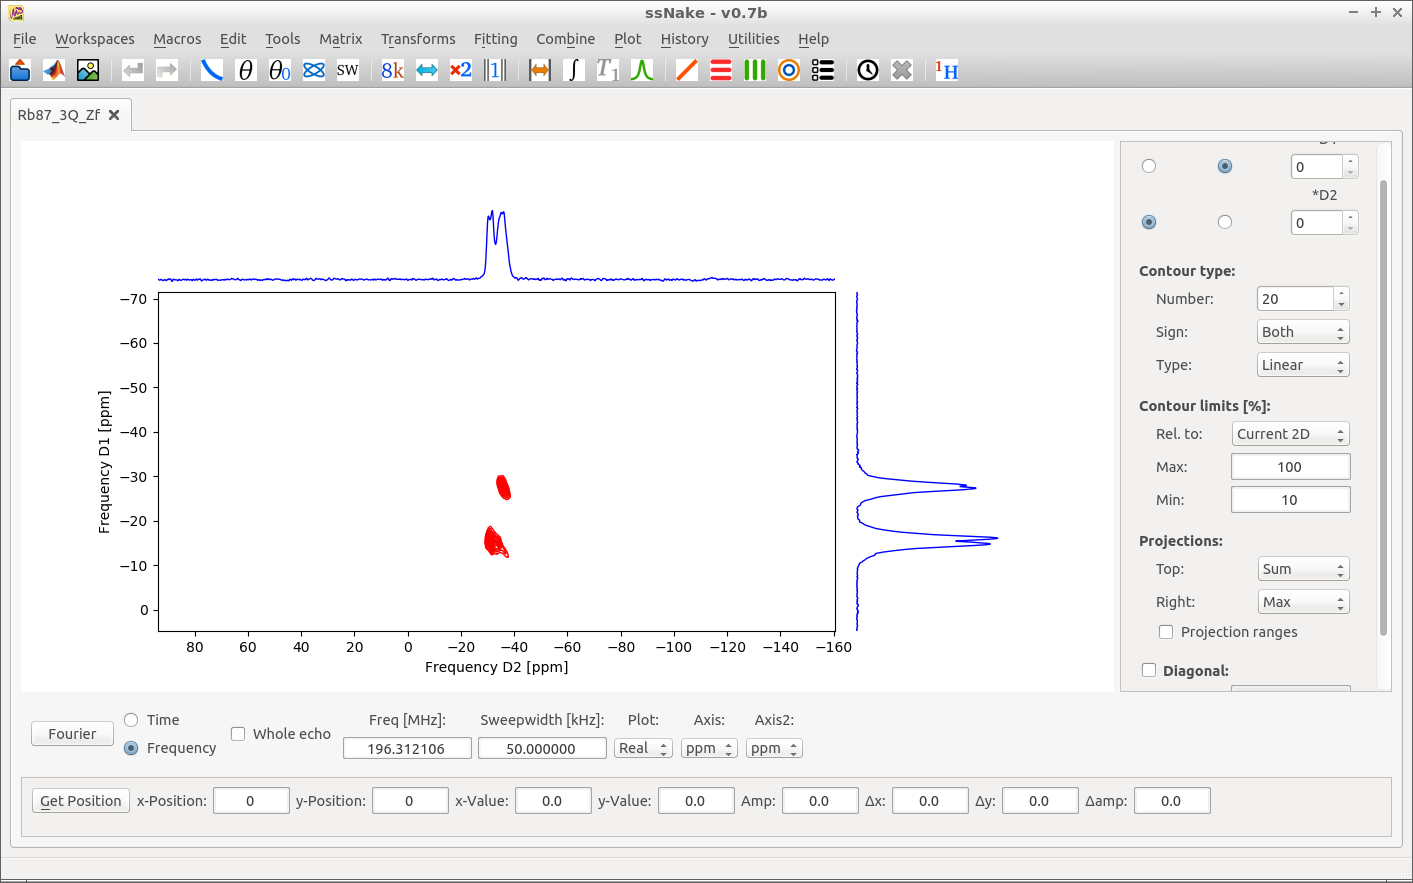
\includegraphics[width=0.8\linewidth]{Figs/Fig5.png}
\end{center}
And zoomed:
\begin{center}
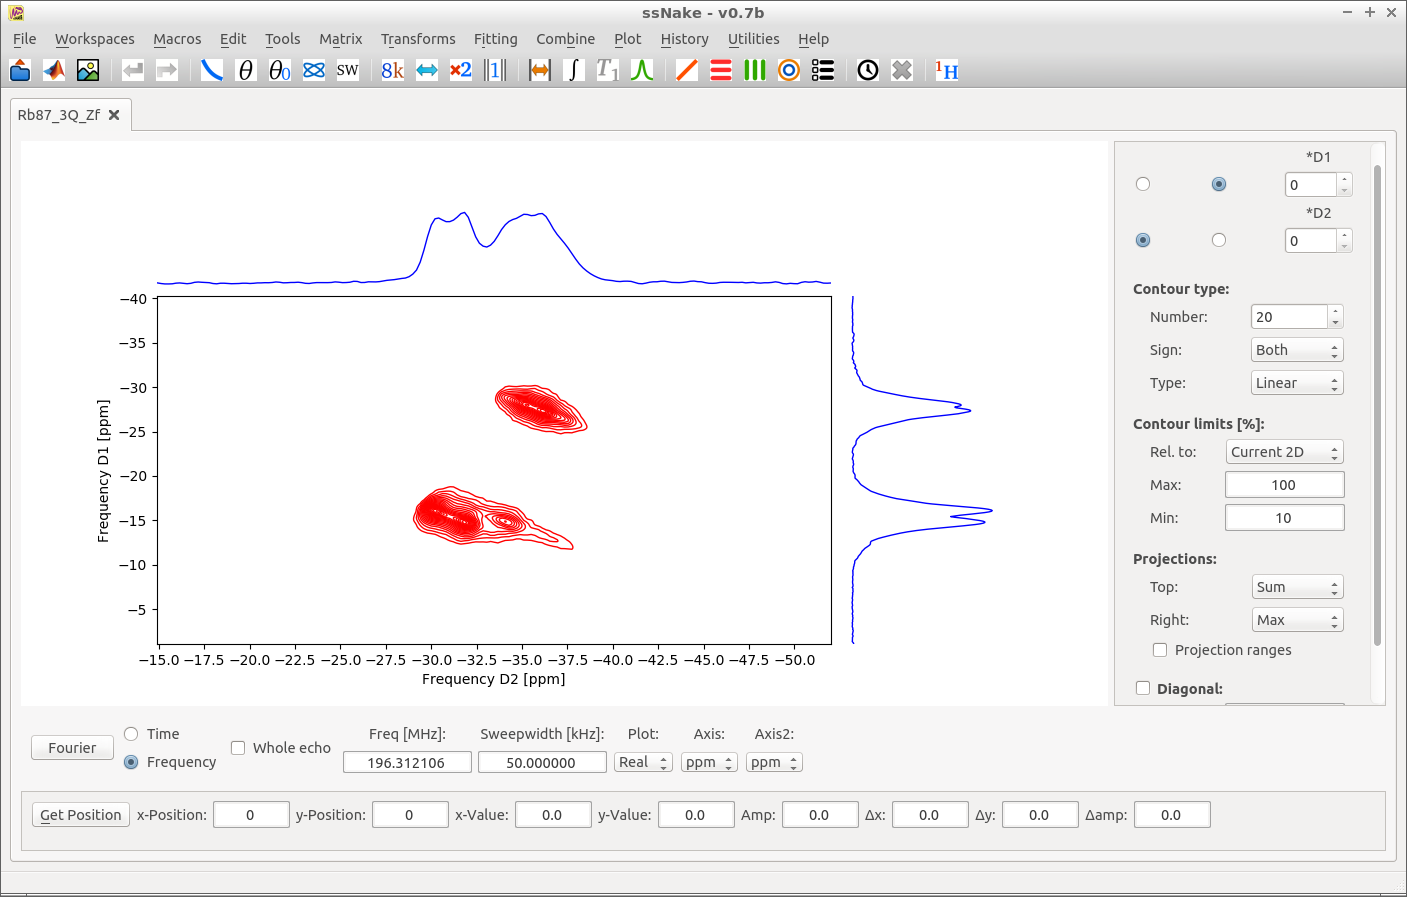
\includegraphics[width=0.8\linewidth]{Figs/Fig6.png}
\end{center}
Note that I put the right projection to `Max' instead of the standard `Sum'. This gives a skyline
projection, which is less influenced by the noise regions of the data.

As can be seen, the different powder patterns are all tilted, going from bottom right to top left.
This is normal for a $z$-filter MQMAS, but needs to be corrected by shearing the spectrum.
\begin{itemize}
	\item Shear via Matrix $\longrightarrow$ Shearing, using the `Spin 3/2, -3Q' setting, and
	  direction `1' and axis '2'
\end{itemize}
This shows (zoomed):
\begin{center}
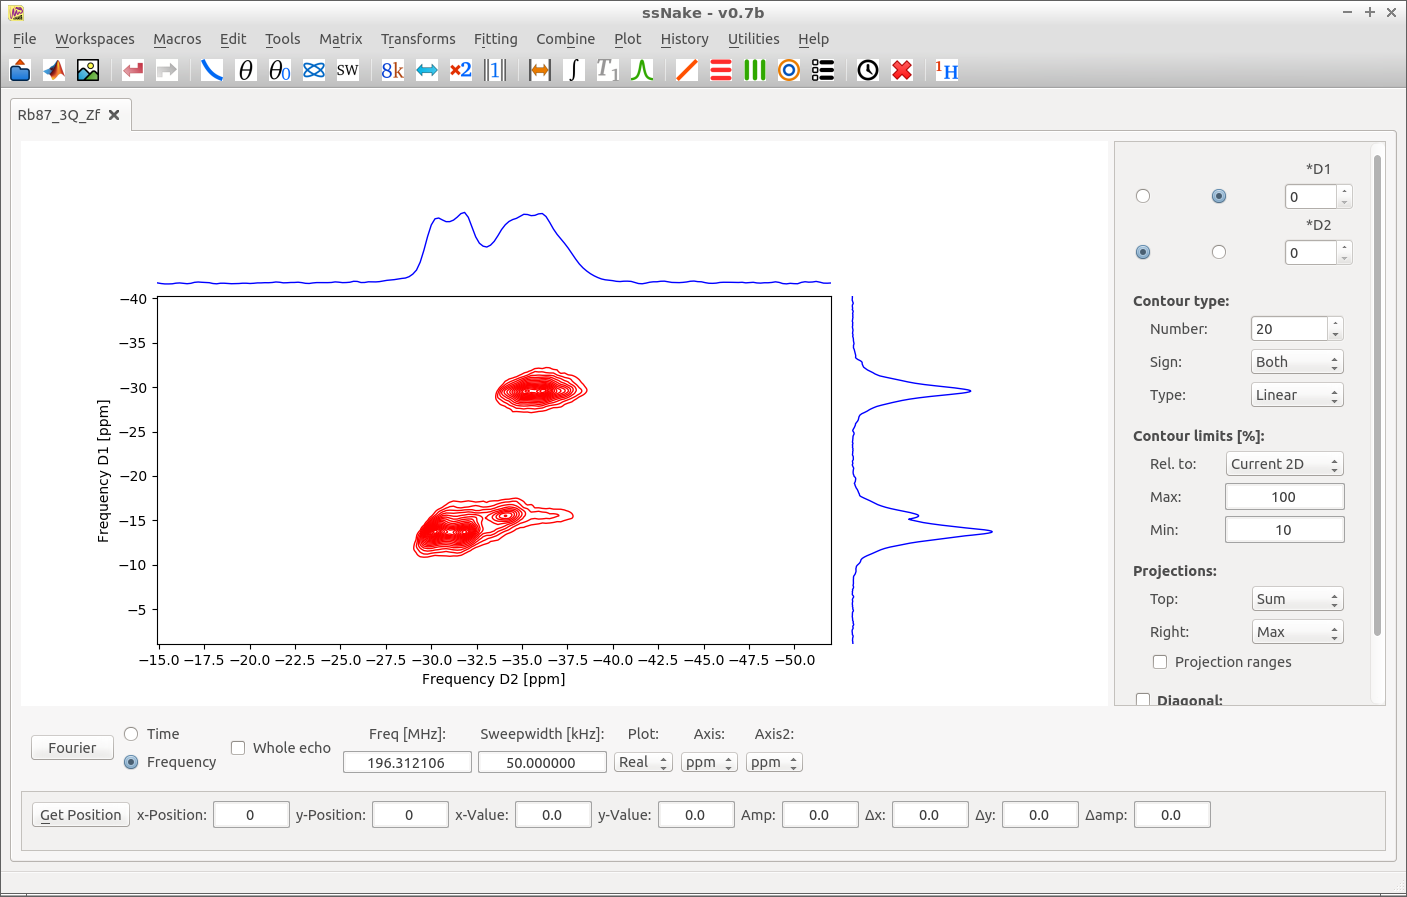
\includegraphics[width=0.8\linewidth]{Figs/Fig7.png}
\end{center}
Which is a nice spectrum! This is the final figure, we now only need to do some work on the axes.

In the view that we have now, the indirect dimension is called the `isotropic' axis. The position
along this axis is determined by the scaled isotropic chemical shift, and the scaled quadrupolar
induced shift. However, it is more convenient to have in axis with the unscaled isotropic chemical
shift. To accomplishing this, we must dived the spectral width by a specific value (which depends on
the spin quantum number).
\begin{itemize}
	\item Switch to D1 (sideframe, click on the upper left radiobutton)
	\item Use Tools  $\longrightarrow$ Scale SW, and select `Spin 3/2, -3Q' and apply
\end{itemize}
Now, we have scaled this axis. As a last step, we must apply a chemical shift reference. This was
measured using a rubidium nitrate solution. Based on this 0 ppm is at: 196.3182865 MHz.
\begin{itemize}
  \item Set the reference via Plot $\longrightarrow$ Reference $\longrightarrow$ Set Reference, and
	 fill in `196.3182865' in the Frequency box
	\item Switch to D2 (sideframe, click on the lower left radiobutton)
	\item Set the reference in the same way
\end{itemize}
This is the final spectrum, and looks like (zoomed):
\begin{center}
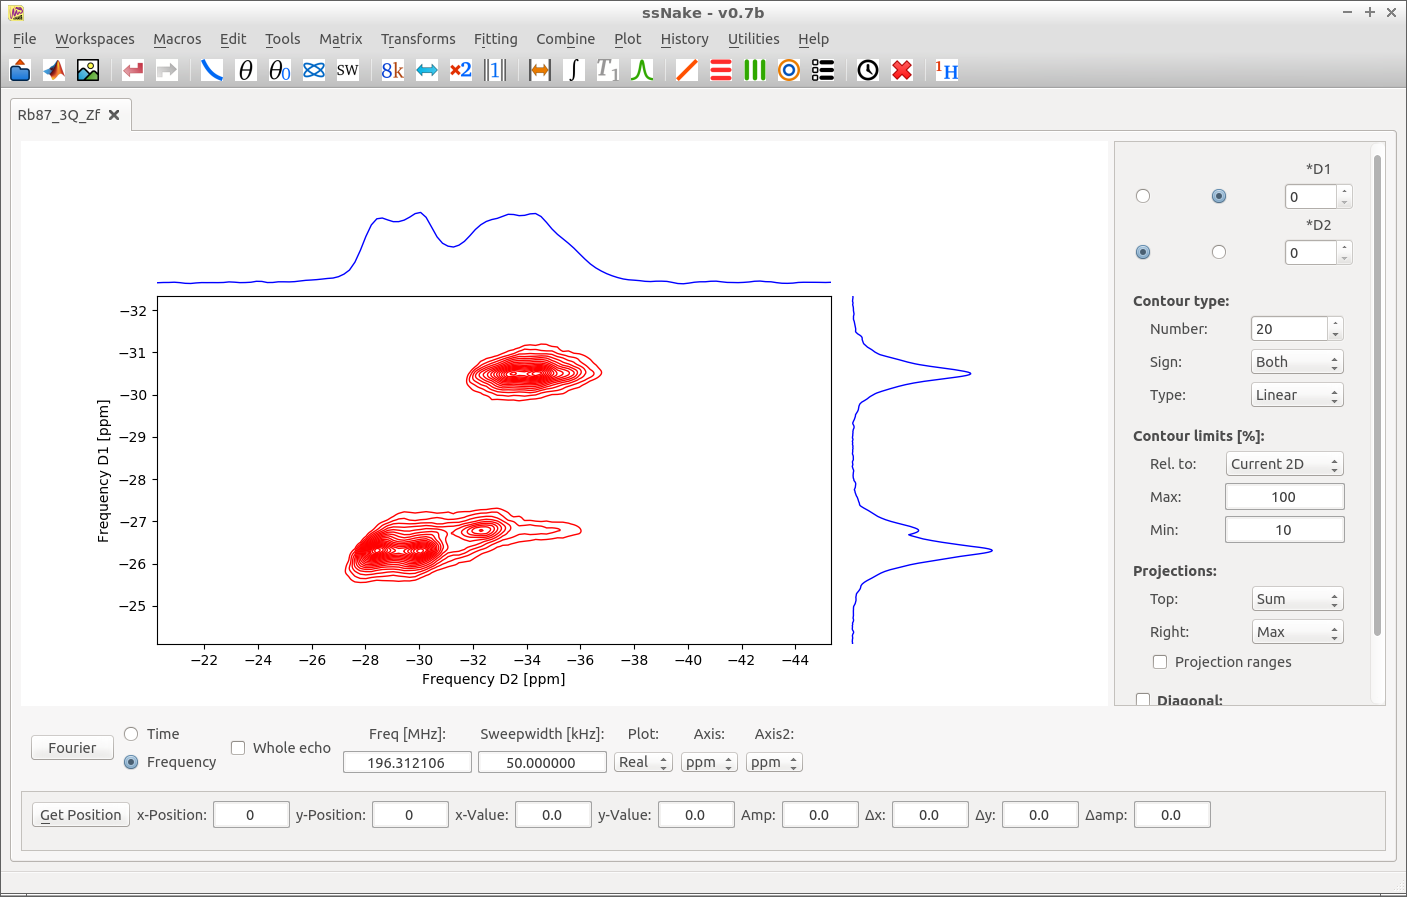
\includegraphics[width=0.8\linewidth]{Figs/Fig8.png}
\end{center}
This spectrum is also delivered with this tutorial, and named `Rb87\_3Q\_Zf\_(final\_spectrum).mat'.
Note that I extracted the relevant region before saving (to lower the file size).
 
Now, we can fit this spectrum. Either by fitting a specific trace with a regular second order
quadrupolar line, or by fitting the whole MQMAS. Another alternative is to only get the isotropic
shift and the quadupolar product $P_\text{Q} = C_\text{Q}\sqrt{1+\eta^2/3}$. For this, we must het
the Centre of Mass for each site, in both D1 and D2. This can be going to the relevant slice,
and using Fitting  $\longrightarrow$ Centre of Mass. Note that in D1, the peaks are symmetric, so the highest
point is the centre in this case.

\begin{center}
  \begin{tabular}{c|cc| c c}
	 \toprule
	 Site & $\delta_1$ [ppm]& $\delta_2$ [ppm]& $\delta_\text{iso}$ [ppm]& $P_\text{Q}$ [MHz]  \\
	 \midrule
	 1 & $-30.5$ & $-34.17$ & $-31.86$ & 1.89 \\
	 2& $-26.8$ &$-31.96$  &$-28.71$ & 2.24\\
	 3& $-26.3$ &$-29.76$ & $-27.58$ & 1.83 \\
	\bottomrule
  \end{tabular}
\end{center}
The last two columns have been calculated using the MQMAS Extraction utility (see the Utilities
menu). 


\section{Split \textit{T}$_\text{1}$ processing}
In a split $T_\text{1}$ experiment, the additional shift of the echo is taken into account within
the pulse sequence. This leads to regular echo data, were the position of the echo in the time
domain is always the same. Due to this, no shearing is required. Also, the data is recorded in such
a way that no hypercomplex processing is necessary. The following assumes that you read the
information above (about the $z$-filter processing).

\begin{itemize}
	\item Open the Varian file Rb87\_3Q\_splitt1.fid using File $\longrightarrow$ Open
\end{itemize}
Now, we must process this data as a whole echo acquisition (see the tutorial on this).

\begin{itemize}
	\item Swap the echo at position 375 (Tools $\longrightarrow$ Swap Echo)
	\item Set the size to 4096 points (Matrix $\longrightarrow$ Sizing)
	\item Apply apodization if required (not used in this case)
	\item Fourier Transform
	\item Phase the imaginary part to zero (168.9 degrees, via Tools $\longrightarrow$ Phasing)
\end{itemize}
This should show (zoomed):
\begin{center}
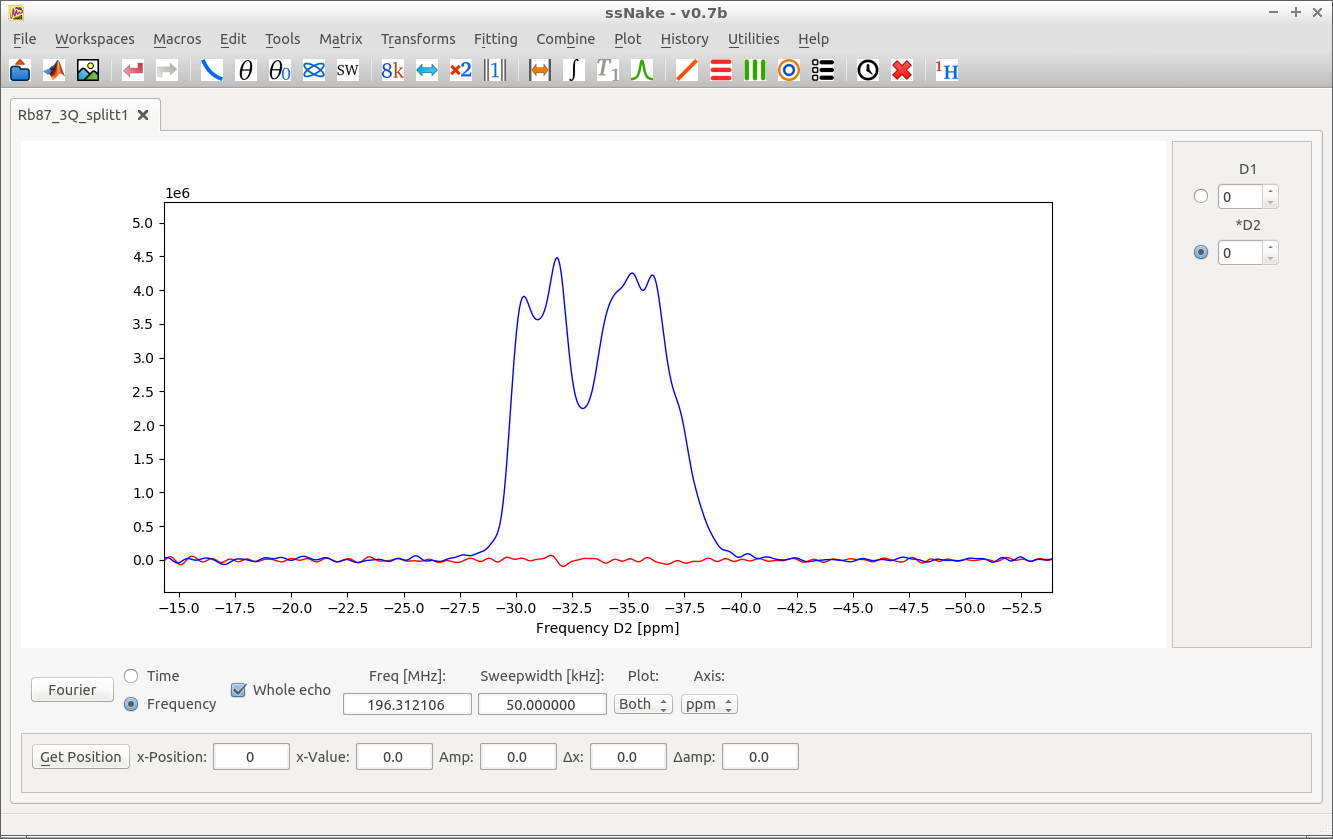
\includegraphics[width=0.8\linewidth]{Figs/Fig9.png}
\end{center}
Now we can process D1:

\begin{itemize}
	\item Switch to D1 (sideframe, radiobutton)
	\item View position 2081 along D2
	\item Tools $\longrightarrow$  Complex Conjugate
	\item Set size to 512
	\item Fourier Transform
\end{itemize}
This gives:
\begin{center}
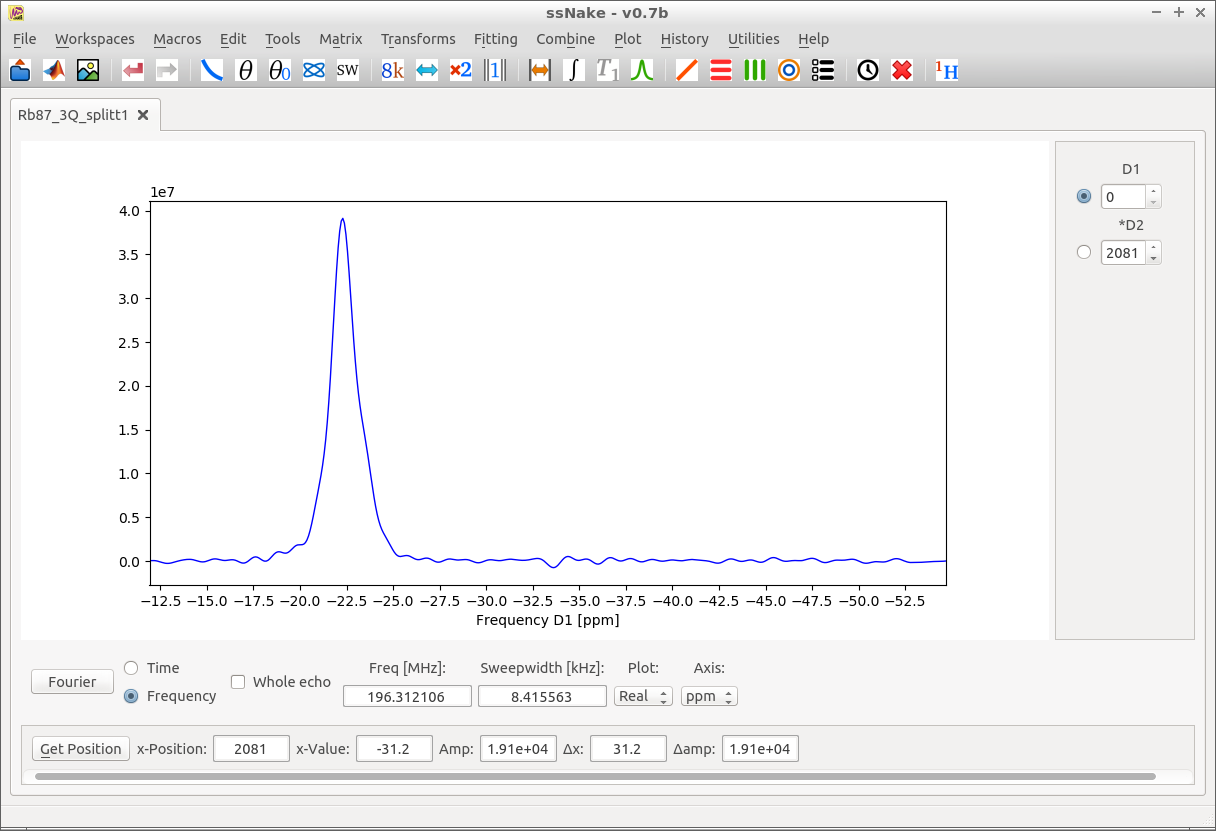
\includegraphics[width=0.8\linewidth]{Figs/Fig10.png}
\end{center}

Now, me must scale the spectral width of this dimension, as was described above. However, with this
experiment some weird stuff is going on. According to the Varian pulse sequence used to measure this
data, the SW that you need to supply must be $9/16$ times the desired spectral width. For the
processing, this means that this scaling must first be undone.

\begin{itemize}
	\item Multiply the spectral width by 16.0/9.0 (either via Tools  $\longrightarrow$ Scale SW, or
	  by typing at the SW box in the bottom frame).
	\item Multiply the SW by the MQMAS scaling value: Tools  $\longrightarrow$ Scale SW, and select `Spin 3/2, -3Q'
\end{itemize}
Now, we must reference the ppm axis in both dimension. As before:
\begin{itemize}
  \item Set the reference via Plot $\longrightarrow$ Reference $\longrightarrow$ Set Reference, and
	 fill in `196.3182865' in the Frequency box
	\item Switch to D2 (sideframe, click on the lower left radiobutton)
	\item Set the reference in the same way
\end{itemize}
Switching to a contour plot gives (zoomed):
\begin{center}
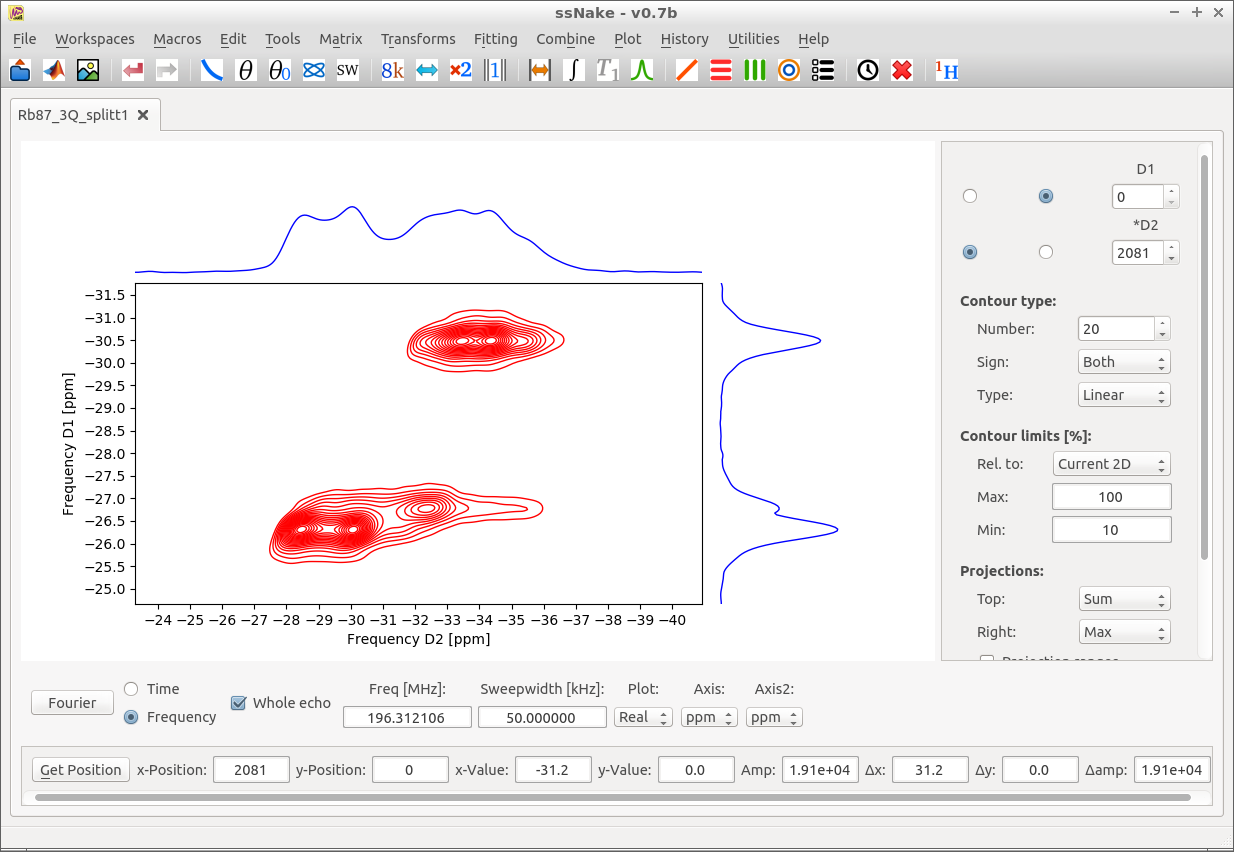
\includegraphics[width=0.8\linewidth]{Figs/Fig11.png}
\end{center}
This is an equivalent spectrum as obtained above, for the $z$-filter data.
This spectrum is also delivered with this tutorial, and named `Rb87\_3Q\_splitt1\_(final\_spectrum).mat'.
Note that I extracted the relevant region before saving this file (to lower the file size).


\section{Equations}
The following Section will show some equations for the relevant shearing and scaling constant used
for MQMAS processing.\footnote{This sections is based on:
  P.\ P.\ Man, \textit{Phys.\ Rev.\ B}, \textbf{5}, 2764 (1998) and 
  T.\ Anup\~{o}ld, A.\ Reinhold, P.\ Sarv, A.\ Samoson, \textit{Solid State Nucl.\ Magn.\ Reson.},
  \textbf{13}, 87 (1998).
  }

These are all included in ssNake in such a way that there is no need to know
these values, or to type them in (as the relative input windows know them). However, for the sake of
completeness, they are provided here.

The following table summarises the values:
\begin{center}
\begin{tabular}[h]{c r r r r}
  \toprule
  $I$ & p$Q$ & $k$ & 1/$a$ & $z$\\
  \midrule
  3/2 & $-3Q$ & 7/9 & 9/34 & 680/27\\
  5/2 & $3Q$ & 19/12 & $-12/17$& 8500/81\\
   & $-5Q$ & 25/12 &12/85& 8500/81 \\
  7/2 & $3Q$ & 101/45 & $-45/34$& 6664/27 \\
   & $5Q$ & 11/9 & $-9/34$ & 6664/27\\
   & $-7Q$ & 161/45 & $45/476$ & 6664/27\\
  9/2 & $3Q$ & 91/36 &  $-36/17$ & 1360/3 \\
   & $5Q$ & 95/36 & $-36/85$ & 1360/3 \\
	& $7Q$ & 7/18 & $-18/117$ & 1360/3 \\
	& $-9Q$ & 31/6 & 6/85 & 1360/3 \\
  \bottomrule
\end{tabular}
\end{center}
Here, $k$ is the shearing factor, $1/a$ the scaling of the spectral width, and $z$ a value necessary
to calculate the quadrupolar product $P_\text{Q}$ from an MQMAS spectrum (see later). The equations
are:
\begin{equation}
  k = p \frac{36I(I+1)-17p^2 - 10}{36I(I+1) - 27}
\end{equation}
\begin{equation}
  1/a = 1/(k - p)
\end{equation}
  \begin{equation}
	 z = \frac{1}{\frac{b}{a}-r}
  \end{equation}
  With:
 \begin{equation}
	b = r	(k + \lambda)
 \end{equation}
 and
 \begin{equation}
	r = -\frac{3}{10}\frac{I(I+1)-3/4}{[2I(2I-1)]^2}
 \end{equation}
 \begin{equation}
	\lambda = p \frac{I(I+1)-3/4 \cdot p^2}{-I(I+1)+3/4}
 \end{equation}

 \subsection{Further background}
 Here, we will quickly derive the relevant equations shown above.

 The centre of mass of the MQMAS data in D2 is:
 \begin{equation}
	\delta_\text{D2} = \delta_\text{iso} + \delta_\text{QIS}  =  \delta_\text{iso} + r
	\frac{P_\text{Q}^2}{\nu_0^2} \cdot 10^6
 \end{equation}
 with
 \begin{equation}
	r = -\frac{3}{10}\frac{I(I+1)-3/4}{[2I(2I-1)]^2}
 \end{equation}
 In D1, before the shearing it is:
 \begin{equation}
	\delta_\text{D1} = -p\delta_\text{iso} + \delta_\text{QIS}  =  -p\delta_\text{iso} +
	\lambda r
	\frac{P_\text{Q}^2}{\nu_0^2} \cdot 10^6
 \end{equation}
 with:

 \begin{equation}
	\lambda = p \frac{I(I+1)-3/4 \cdot p^2}{-I(I+1)+3/4}
 \end{equation}
After shearing, this becomes:
 \begin{align}
	\delta_\text{D1'} &= \delta_\text{D1} + k\delta_\text{D2} = (k - p)\delta_\text{iso} +
	r	(k + \lambda) \frac{P_\text{Q}^2}{\nu_0^2} \cdot 10^6 \\
	& = a  \delta_\text{iso} + b \frac{P_\text{Q}^2}{\nu_0^2} \cdot 10^6
 \end{align}
 with the constants:
 \begin{align}
	a & = k(I,p) - p \\
	b & = r(I)	(k(I,p) + \lambda(I,p))
 \end{align}
 A good way to processes this data, is to divide the spectral width of F1 by $a$. This leads to a
 chemical shift axis, were a increase in the isotropic shift of a line leads to an exact same change
 in the F1 dimension. This leads to:
 \begin{equation}
	\delta_\text{D1''} = \delta_\text{iso} + \frac{b}{a} \frac{P_\text{Q}^2}{\nu_0^2} \cdot 10^6
 \end{equation}
 When this processing is performed, nuclei that experience a quadrupolar coupling always lay in the
 lower right part of the spectrum, lower than the diagonal that is. If a lineshape is fully on the
 diagonal, but stretched along it, there is a chemical shift distribution.

 Based on the centre off mass in D1'' and D2, the NMR parameters $\delta_\text{iso}$ and $P_\text{Q}$
 can be extracted:

 \begin{align}
	\delta_\text{iso} & = \delta_\text{D1''} - \frac{b}{a\cdot r} \delta_\text{D2} =
	\delta_\text{D1''} - \frac{k+\lambda}{a} \delta_\text{D2} \\
	& = \frac{17 \delta_\text{D1''} + 10  \delta_\text{D2}}{27}
 \end{align}
 This result is the same for any $I$ and $p$.

 For $P_\text{Q}$ the case is more difficult:
 \begin{align}
	\delta_\text{D1''} - \delta_\text{D2} =& \left( \frac{b}{a} - r \right)
	\frac{P_\text{Q}^2}{\nu_0^2} \cdot 10^6\\ 
	P_\text{Q} =& \sqrt{  \frac{1}{\frac{b}{a}-r}\cdot 10^{-6} \nu_0^2 (\delta_\text{F1''} -
	\delta_\text{F2}) } \\
	=& \sqrt{  z \cdot 10^{-6} \nu_0^2 (\delta_\text{F1''} -
	\delta_\text{F2}) } 
  \end{align}
  With the scaling factor:
  \begin{equation}
	 z = \frac{1}{\frac{b}{a}-r}
  \end{equation}
  These depend only on $I$ and are tabulated above. These equation can be used to calculate the
  isotropic shift and quadrupolar product ($P_\text{Q}$) of a line based on the centre of mass of
  the line along both dimension. These equations have been included in ssNake in the form of a
  utility. See the Utilities menu.


\end{document}
